\section{Model to Code Transformations}

\subsection{Rationale}

\frame {
  \frametitle{Rationale---Why generate it automatically?}
  \begin{itemize}
    \item Ada Ravenscar, more tedious than meets the eye
    \item Code generation will reduce this effort
    \item Will result in no (or fewer) errors in the code generated
    \item AADL and Ada Ravenscar, a good \emph{fit}
      \begin{itemize}
        \item Domain specifity of AADL
        \item Intuitive meshing AADL/Ravenscar, similar ``concept
          space''
        \item Industrial acceptance
        \item Reasonable level of abstraction \pause \emph{Yes, I
          explain}
      \end{itemize}
  \end{itemize}
}

\frame {
  \frametitle{Generation of an execution framework}
  \begin{itemize}
    \item AADL system constructs$\implies$``execution
      framework''
    \item \textcolor{gray}{Something like Statecharts
      (functional)$\implies$sequential code}
    \item Framework consists of the runtime entities (process, thread)
    \item Entities respond to non-functional requirements of system
      \begin{itemize}
        \item Tasks with correct temporal characteristics
        \item Inter-task communication buffers
        \item Interfaces of various parts as described in the
          architecture
      \end{itemize}
  \end{itemize}
}

\frame {
  \frametitle{Ravenscar Meta-model (RMM)}
  \begin{itemize}
    \item Ravenscar not patterns, but need decisions for automation
    \item These decisions resulted in domain model, the RMM
    \item Intermediate, internal model
    \item Workflow: $AADL_{instance}\to RMM_{instance}\to Ada$
  \end{itemize}
  \ \ \ \ \ \ \ \ \ \ \ \ \ \ \ \ \ \ \ \ \ \ $PSM_1$\ \ \ \ \ \ \ \ \ \ \ \ \ $PSM_2$
  \ \ \ \ \ \ \ \ \ Code
}

\frame {
  \frametitle{Glimpse at the RMM}
  $\includegraphics[scale=0.5]{../figs/tasking_config}$
}

\subsection{Generated execution framework}

\frame {
  \frametitle{Overview of transformations}
  \begin{itemize}
    \item Process$\to$Ada main compilation unit
    \item Periodic and sporadic thread$\to$Ada task
    \item Data ports$\to$Ada protected objects
    \item Event and event data ports$\to$Ada protected objects with
      entry
    \item Data component$\to$Ada type
    \item Data subcomponent$\to$Ada PO, package or variable
    \item Subprogram$\to$Ada procedure
  \end{itemize}
}

\frame {
  \frametitle{Transformation example---Periodic thread}
  \begin{center}
    $\includegraphics[scale=0.65]{../figs/thread2task}$
  \end{center}
}

\frame {
  \frametitle{Transformation example---Data ports}
  \begin{itemize}
    \item Transformed to special PO named exchangers
    \item Single internal value, concurrency safe access
  \end{itemize}
  \pause
  \begin{center}
  $\includegraphics[scale=0.5]{../figs/dataports_presentation}$
  \end{center}
}

\frame {
  \frametitle{Transformation example---Event ports}
  \begin{itemize}
    \item Transformed to one enumeration, and a \alert{synchronizer}
      PO
    \item Procedures send events, entry retreives event type
  \end{itemize}
  \pause
  $\includegraphics[scale=1.0]{../figs/synchronizer}$
}

\frame {
  \frametitle{Transforms---Sporadic thread}
  $\includegraphics[scale=0.6]{../figs/sync_transform}$
}

\frame {
  \frametitle{ARC---Implementation of transformations}
  \begin{itemize}
    \item Open source Eclipse plugin
    \item Uses the OSATE AADL parser
    \item Validate incoming AADL model for conversion
    \item Transform AADL model into an instance of RMM
    \item Traverse RMM instance to emit Ada code
  \end{itemize}
  $\includegraphics[scale=0.5]{../figs/ARC_process}$
}

\subsection{Example of utilization}

\frame {
  \frametitle{Example case}
  \begin{itemize}
    \item A small example to illustrate use and usability
    \item Model the HCI \& a monitoring task for a small aircraft
    \item Sensors and operator are to be simulated
    \item If sensors give values outside tolerance, raise alarm
    \item If engine fails, raise alarm
  \end{itemize}
}

\frame {
  \frametitle{Design}
  $\includegraphics[scale=0.4]{../figs/caseStudy}$
}

\frame {
  \frametitle{Observations}
  \begin{itemize}
    \item All tasking code automatically generated
    \item Inter-task communication framework automatically generated
    \item Callback skeletons automatically generated
    \item API to the port features was generated
    \item Only part written by hand: callback bodies, i.e.,
      \begin{itemize}
      \item Execution framework---tasks, data buffers, event
        signaling---automatically generated
      \item Only functional, or algorithmic portion, written by hand
      \end{itemize}
    \item Greatly eased the development process
  \end{itemize}
}


%%%%%%%%%%%%%%%%%%%%%%%%%%%%%%%%%%%%%%%%%%%%%%%55
\begin{comment}
\frame {
  \frametitle{Transforms---Process component}
  \begin{itemize}
    \item An AADL process component is an ``address space''
    \item Transformed to a main compilation unit in Ada
    \item When compiled, results in an executable
    \item Sole purpose of this compilation unit is to include packages
      that declare the tasks and the communication constructs it
      contains
    \item It then goes into an infinite loop and serves as the idle
      task
  \end{itemize}
}

\frame {
  \frametitle{Transforms---Data components}
  \begin{itemize}
    \item All data component types and implementations are transformed
      to Ada types
    \item Data components may be of two varieties: primitive or
      compound
    \item A primitive data component is one which has no subcomponents
    \item Primitive data components are transformed to Ada types via
      an analysis of their property \texttt{Data\_Type}
      \begin{itemize}
        \item \texttt{Integer}
        \item \texttt{Boolean}
        \item \texttt{Char}
        \item $\ldots$
      \end{itemize}
    \item Compound data components are transformed to Ada records,
      with each member of the record construct corresponding to the
      subcomponents of the data component in question
  \end{itemize}
}

\frame[containsverbatim] {
  \frametitle{Transforms---Data components (contd.)}
  \begin{minipage}{0.45\linewidth}
    \begin{lstlisting}[language=aadl]
data Int_Type
properties
  Data_Type => Integer;
end Int_Type;

data Int_Vector
properties
  Data_Type => Integer;
  Length => 10;
end Int_Vector;
    \end{lstlisting}
  \end{minipage}
  \hspace{2mm}
  \begin{minipage}{0.45\linewidth}
    \begin{lstlisting}[language=ada]
type Int_Type is new Integer;




type Int_Vector 
     is array (1..10) of Integer;


---------------------------------
    \end{lstlisting}
  \end{minipage}
}

\frame {
  \frametitle{Transforms---Periodic threads}
  \begin{itemize}
    \item Transformed to Ada tasks with the appropriate properties
      \begin{itemize}
        \item Period
        \item Size of the stack
        \item Deadline
        \item Appropriate entrypoint
      \end{itemize}
    \item Even though no dynamic creation allowed, instantiation of
      generic packages is legal, as it takes place at elaboration time
    \item A generic package for a periodic task, containing only an
      instance of a task object
    \item Above-mentioned properties become instantiation parameters
      for the generic package
    \item A ``functional unit'' package is generated for each periodic
      thread, it contains the callback (entrypoint) for that thread
    \item The entrypoint is an annotated procedure in order to
      preserve modifications between code generation operations
  \end{itemize}
}

\frame[containsverbatim] {
  \frametitle{Transforms---Periodic thread example}
%  \begin{minipage}{0.45\linewidth}
    \begin{lstlisting}[language=aadl]
process implementation Partition.Impl
subcomponents
  Sensor_Sim : thread Sensor_Sim_T.RS {
    Period => 20 Ms;
    Source_Stack_Size => 4096 B;
    Compute_Entrypoint => "On_Sensor_Sim";
    Dispatch_Protocol => Periodic;
    Deadline => 15 Ms; };
end Partition.Impl;
    \end{lstlisting}
}

\frame[containsverbatim] {
  \frametitle{Transforms---Periodic thread example (contd.)}
    \begin{lstlisting}[language=ada]
package Sensor_Sim is new 
  Ravenscar_Periodic (
    Period_P => Ada.Real_Time.Milliseconds(20),
    Deadline_P => Ada.Real_Time.Milliseconds(15),
    Priority_P => 239,  
    Stack_Size_P => 4096, 
    Dispatch => Dispatcher.Sensor_Sim_Dispatcher);
    \end{lstlisting}
}

\frame {
  \frametitle{Transforms---Data ports}
  \begin{itemize}
    \item They are the simplest of communication mechanism
    \item Represent a shared state between two components
    \item Have directional semantics (in, out and in out)
    \item Have a data type associated with them (their
      \emph{classifier})
    \item AADL semantics allow fan-out (multiple destinations), but
      not fan-in (multiple sources) for data ports
  \end{itemize}
  \pause
  $\includegraphics[scale=0.4]{../figs/comp_code}$
}

\frame {
  \frametitle{Transforms---Data ports (contd.)}
  \begin{itemize}
    \item Transformed to a specific type of protected object named
      \alert{exchanger}
      \begin{itemize}
        \item No entry
        \item Two procedures, \texttt{Get\_Value} \&
          \texttt{Set\_Value}
        \item An internal data member of the same type as the port's
          classifier
        \item A Boolean to keep track of internal data value's freshness
      \end{itemize}
    \item The two procedures allow concurrency safe access to the
      internal data for both components (normally threads)
    \item This exchanger is \emph{always} associated to the \texttt{in
      data port}
    \item All exchangers for a process are instantiated in a single
      package, an API is generated in the functional unit package of
      each thread that participates in a port communication
  \end{itemize}
}

\frame {
  \frametitle{Transforms---Data ports example}
  $\includegraphics[scale=0.5]{../figs/dataports_presentation}$
}

\frame {
  \frametitle{Transforms---Sporadic threads \& events}
  \begin{itemize}
    \item Sporadic threads are event triggered
    \item In AADL, signified by effective property association
      \texttt{Dispatch\_Policy => Sporadic}
    \item Must have \emph{at least} one incoming event or event data
      port
    \item No entrypoint associated specifically with the thread
    \item One entrypoint is associated with \emph{each} incoming event
      and event data port
    \item The \texttt{Period} property is taken to signify the minimum
      inter-arrival time for successive jobs
  \end{itemize}
}

\frame {
  \frametitle{Transforms---Sporadic threads \& events}
  \begin{itemize}
    \item An enumeration generated for each incoming event
    \item Each sporadic thread is transformed to an Ada task with
      minimum inter-arrival time restriction
    \item A special protected object named \emph{synchronizer} is
      generated per sporadic thread
      \begin{itemize}
        \item An entry \texttt{Await\_Event} on which the sporadic
          task will wait
        \item A set of procedures \texttt{Send\_<Port\_Name>} and
          \texttt{Send\_<Port\_Name> (D : in <Port\_Classifier>)}
        \item A set of procedures \texttt{Get\_<Port\_Name> (D : out
          <Port\_Type>)}
        \item A circular queue that stores event types
        \item A circular queue per incoming \emph{event data port}
      \end{itemize}
    \item Strict one-to-one relation between sporadic thread \&
      synchronizer
    \item Restriction coming from RMM, not from Ravenscar Profile
  \end{itemize}
}

\frame {
  \frametitle{Transforms---Sporadic thread$\to$Synchronizer}
  $\includegraphics[scale=1.0]{../figs/synchronizer}$
}

\frame {
  \frametitle{Transforms---Sporadic thread}
  $\includegraphics[scale=0.6]{../figs/sync_transform}$
}

\subsection{Example of utilization}

\frame {
  \frametitle{Problem statement}
  \begin{itemize}
    \item A small example to illustrate use and usability
    \item Model the HCI \& a monitoring task for a small aircraft
    \item Sensors and operator are to be simulated
    \item If attitude sensors give values outside tolerable intervals,
      raise alarm
    \item If engine fails, raise alarm
  \end{itemize}
}

\frame {
  \frametitle{Design}
  $\includegraphics[scale=0.4]{../figs/caseStudy}$
}


\frame {
  \frametitle{ARC}
  \begin{itemize}
    \item Open source Eclipse plugin
    \item Uses the OSATE AADL parser
    \item Performs validation on the incoming AADL model to ensure it
      \emph{can} be transformed to Ravenscar-compliant code
    \item Transforms the AADL model into an instance of the RMM
    \item Traverses the RMM instance to emit Ada code
  \end{itemize}
  $\includegraphics[scale=0.5]{../figs/ARC_process}$
}

\frame {
  \frametitle{Observations}
  \begin{itemize}
    \item All tasking code was automatically generated
    \item The entire inter-task communication framework was
      automatically generated
    \item The callback procedures' skeletons were automatically
      generated
    \item An API corresponding to the port features on each thread's
      interfaces was generated
    \item Only part written by hand was callback procedure bodies,
      i.e.
      \begin{itemize}
      \item Execution framework---tasks, data buffers, event
        signaling---automatically generated
      \item Only functional, or algorithmic portion, written by hand
      \end{itemize}
    \item Greatly eased the development process
  \end{itemize}
}

\end{comment}
%%%%%%%%%%%%%%%%%%%%%%%%%%%%%%%%%%%%%
